\chapter{Time Management}
This chapter shows the amount of time that went into the project.

\ \\
As can be seen in figure \ref*{fig:timeTracking},
the majority of the time was spent on improving the prototype.
Almost half of the time (178 hours) was spent on refactorings and usability upgrades.
This includes the manual and interactive modes, as well as highlighting text on the terminal and the user interaction overall.

\ \\
Creating the base prototype took around 111 hours,
which includes the research that had to be done about the Core language as well as some Haskell language features that would be used in the project.
The result was a prototype that could do step Haskell automatically but not manually.

\ \\
The documentation also took a good amount of time,
making up for over a sixth of the total time spent, spread over the three last weeks.

\ \\
Meetings with the advisor and other people that are involved in the project took less than 24 hours combined,
which comes to a bit over 1 hour per week.

\ \\
The time spent overall comes to around 383 hours, which equals a weekly workload of around 21 hours and 20 minutes.

\begin{figure}
    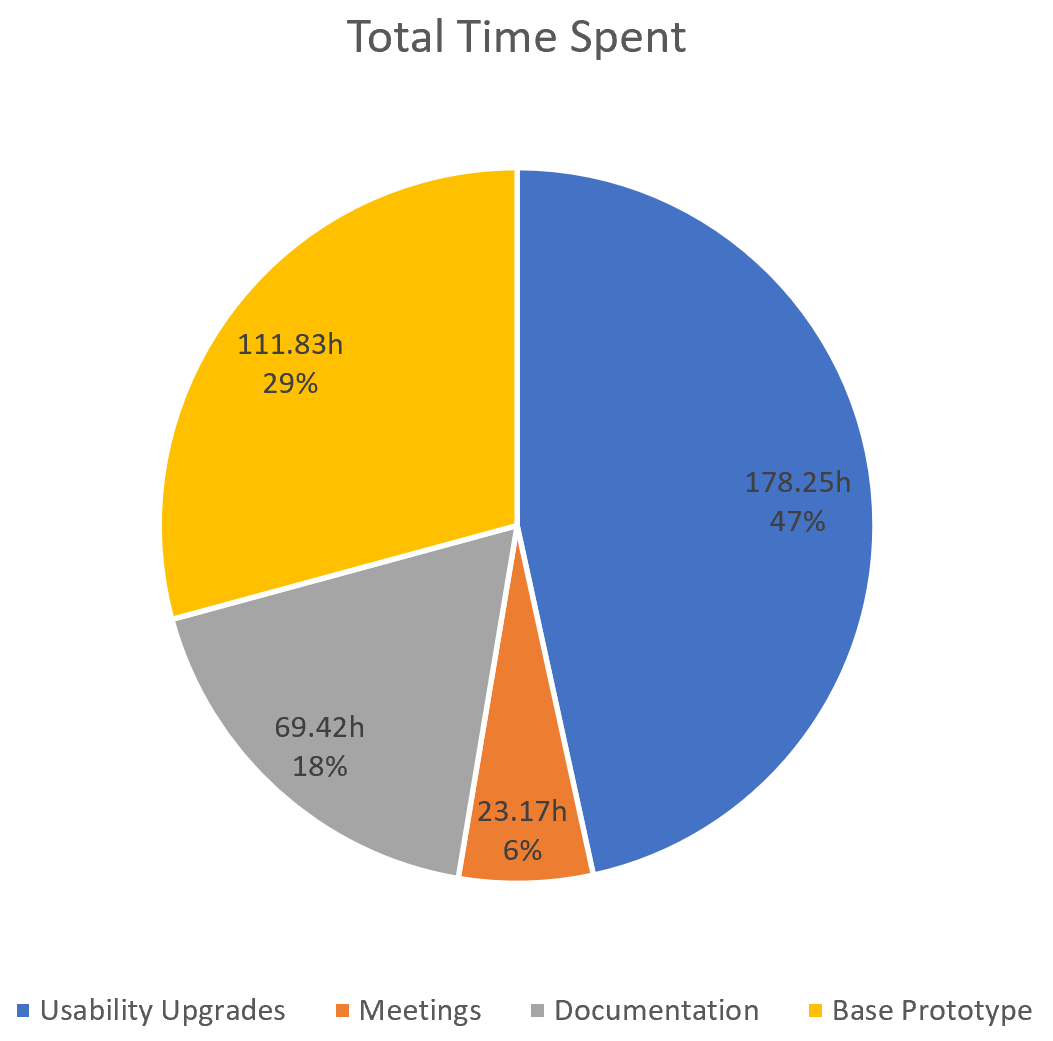
\includegraphics[width=1\textwidth]{resources/time_tracking.PNG}
    \caption{Time spent by epic}
    \label{fig:timeTracking}
\end{figure}
